\newpage %! newpage
\chapter{Ergebnisse der Datenerhebung}

\todo{Kleine Einleitung + 108 Projekte erwähnen.}

\todoo{In den folgenden unterkapitel... werden die Ergebnisse der 108 Projekte ...}

% ------------------------------------------- Lizenzen ------------------------------------------- %
\section{Lizenzen} \label{sec:Ergebnisse_Datenerhebung_Lizenzen}

\todo{Verweis auf Kapitel 2.1 Lizenzen => Warum genau diese Aufteilung}

\bigskip
\noindent
Um die \hyperref[H:1]{Hypothese H1} zu prüfen wurden der Datensatz in Projekte mit freizügigen und
restriktiven
Lizenzen. \todoo{Die Aufteilung erfolgt hierbei, wie im Kapitel 1.3.3.7 zu Lizenzen näher erklärt wurde.}
In der Tabelle \ref{tab:lizenzen} findet sich eine Zusammenfassung aller Lizenzen der
Projekte die erfasst wurden. 91\% der Projekte haben eine freizügige Lizenz, wobei die MIT Lizenz mit 69\%
die beliebteste aller Lizenzen ist.

Um die Gruppen miteinander zu vergleichen wurde der Median der Anzahl der Sterne verwendet, da diese
sehr stark verteilt ist. Der Median für permissive Lizenzen liegt bei 27.515 Sternen, für
restriktive bei 21.595,5. Somit haben Projekte mit permissiven Lizenzen im Median 27,4\% mehr Sterne
als Projekte mit restriktiven Lizenzen.

Aufgrund der großen Mengenunterscheiden zwischen freizügigen und restriktiven Projekten wurde
zusätzlich ein Ranking erstellt. Wie in Abbildung \ref{abb:permissive_vs_restriktiv_BarChart} zu sehen
ist wurden hierfür die Projekte nach Sternen sortiert. Von 108 ausgewerteten Projekten liegt das erste
mit restriktiver Lizenz auf Platz 35, das heißt die \todoo{Top} 31\% der Projekte sind alle 
permissiv lizenziert. Projekte mit freizügigen Lizenzen übertreffen die restriktiven sowohl in der Menge 
als auch in der Beliebtheit.
 




% \bigskip
% \noindent
% % Top 100 Projekte
% Um auszuschließen das es sich hierbei, um ein Phänomen handelt welches sich nur bei den
% Programmiersprachen JS/TS wiederfindet wurden, wie in \ref{sec:top_100_projects} beschrieben,
% die Top 100 GitHub Projekte separat erfasst. Wie sich in Tabelle \ref{tab:top_100}
% zeigt ist die MIT Lizenz mit 58\% die am häufigsten verwendete Lizenz gefolgt von Apache 2.0 (24\%)
% und der BSD-3-Clause (8\%).
% Insgesamt sind 93\% der Top 100 Projekte auf GitHub permissiv lizenziert.



% ------------------------------------------ Hypothese 2 ----------------------------------------- %
\bigskip
\noindent
Um die zweite Hypothese zu prüfen wurden ebenfalls die Mediane verglichen, allerdings wurden hier
Anzahl der Mitwirkenden sowie Commits der letzten 12 Monate betrachtet. Der Median wurde in diesem
Fall gewählt, da sowohl die Anzahl Commits als die der Mitwirkenden starke Ausreißer haben.

Im Median haben restriktive Projekte 78 Mitwirkende und 74,5 Commits, permissive Projekte haben 274,5
Mitwirkende und 182 Commits.
In einen weiterem Ranking, sortiert nach Mitwirkenden befindet sich das erste Projekt mit
restriktiver Lizenz auf Platz 51. Im Ranking der Anzahl der Commits erreicht,
wie man in Abbildung \ref{abb:license_vs_commits} sehen kann, das erste restriktive Projekt Platz 9.

Im Ranking der Anzahl der Commits befinden sich unter den ersten 20 Projekten zwei OSP mit restriktive
Lizenzen.


% Tabelle: Lizenzen der erfassten Projekte
\begin{table}[h]
    \begin{tabular}{lcllc}
        \cline{1-2} \cline{4-5}
        \textbf{Permissive Lizenz} & \multicolumn{1}{l}{Anz.} & \hspace{2cm} & \textbf{Restriktive Lizenz} & \multicolumn{1}{l}{Anz.} \\ \cline{1-2} \cline{4-5}
        MIT                        & 74                       &              & AGPLv3                      & 4                        \\
        Apache 2.0                 & 18                       &              & GPLv3                       & 3                        \\
        BSD 3-Clause               & 3                        &              & LGPLv2.1                    & 1                        \\
        BSD 2-Clause               & 2                        &              & OSLv3.0                     & 1                        \\
        ISC                        & 1                        &              & LGPLv3                      & 1                        \\ \cline{1-2} \cline{4-5}
        \textit{Gesamt}            & 98                       &              & \textit{Gesamt}             & 10
    \end{tabular}%
    \caption{Lizenzen der erfassten Projekte}
    \label{tab:lizenzen}
\end{table}

% Tabelle aus vom GitHub Blogpost & Top 100
% \begin{table}[]
    \begin{tabular}{clc}
        \hline
        \multicolumn{1}{l}{Rang} & Lizenz      & \multicolumn{1}{l}{\% der Projekte} \\ \hline
        1                        & MIT          & 44,69\%                            \\
        2                        & Other        & 15,68\%                            \\
        3                        & GPLv2        & 12,96\%                            \\
        4                        & Apache       & 11,19\%                            \\
        5                        & GPLv3        & 8,88\%                             \\
        6                        & BSD 3-Clause & 4,53\%                             \\
        7                        & Unlicense    & 1,87\%                             \\
        8                        & BSD 2-clause & 1,70\%                             \\
        9                        & LGPLv3       & 1,30\%                             \\
        10                       & AGPLv3       & 1,05\%
    \end{tabular}%
    \caption{GitHub Blogeintrag: Lizenznutzung 2015}
    \label{tab:GitHub_Blog_Lizenznutzung2015}
\end{table}

\begin{table}[]
    \begin{tabular}{clc}
        \hline
        \multicolumn{1}{l}{Rang} & Lizenz       & \multicolumn{1}{l}{Anzahl der Projekte} \\ \hline
        1                        & MIT          & 58                                      \\
        2                        & Apache       & 24                                      \\
        3                        & BSD 3-Clause & 8                                       \\
        4                        & GPLv3        & 4                                       \\
        5                        & GPLv2        & 2                                       \\
        6                        & BSD 2-Clause & 1                                       \\
        7                        & ISC          & 1                                       \\
        8                        & MLP 2.0      & 1                                       \\
        9                        & AGPLv3       & 1
    \end{tabular}%
    \caption{Lizenzen der Top 100 GitHub Projekte}
    \label{tab:top_100}
\end{table}


% Abbildung: Lizenzen vs Lizenzen
\begin{figure}[]
    \centering
    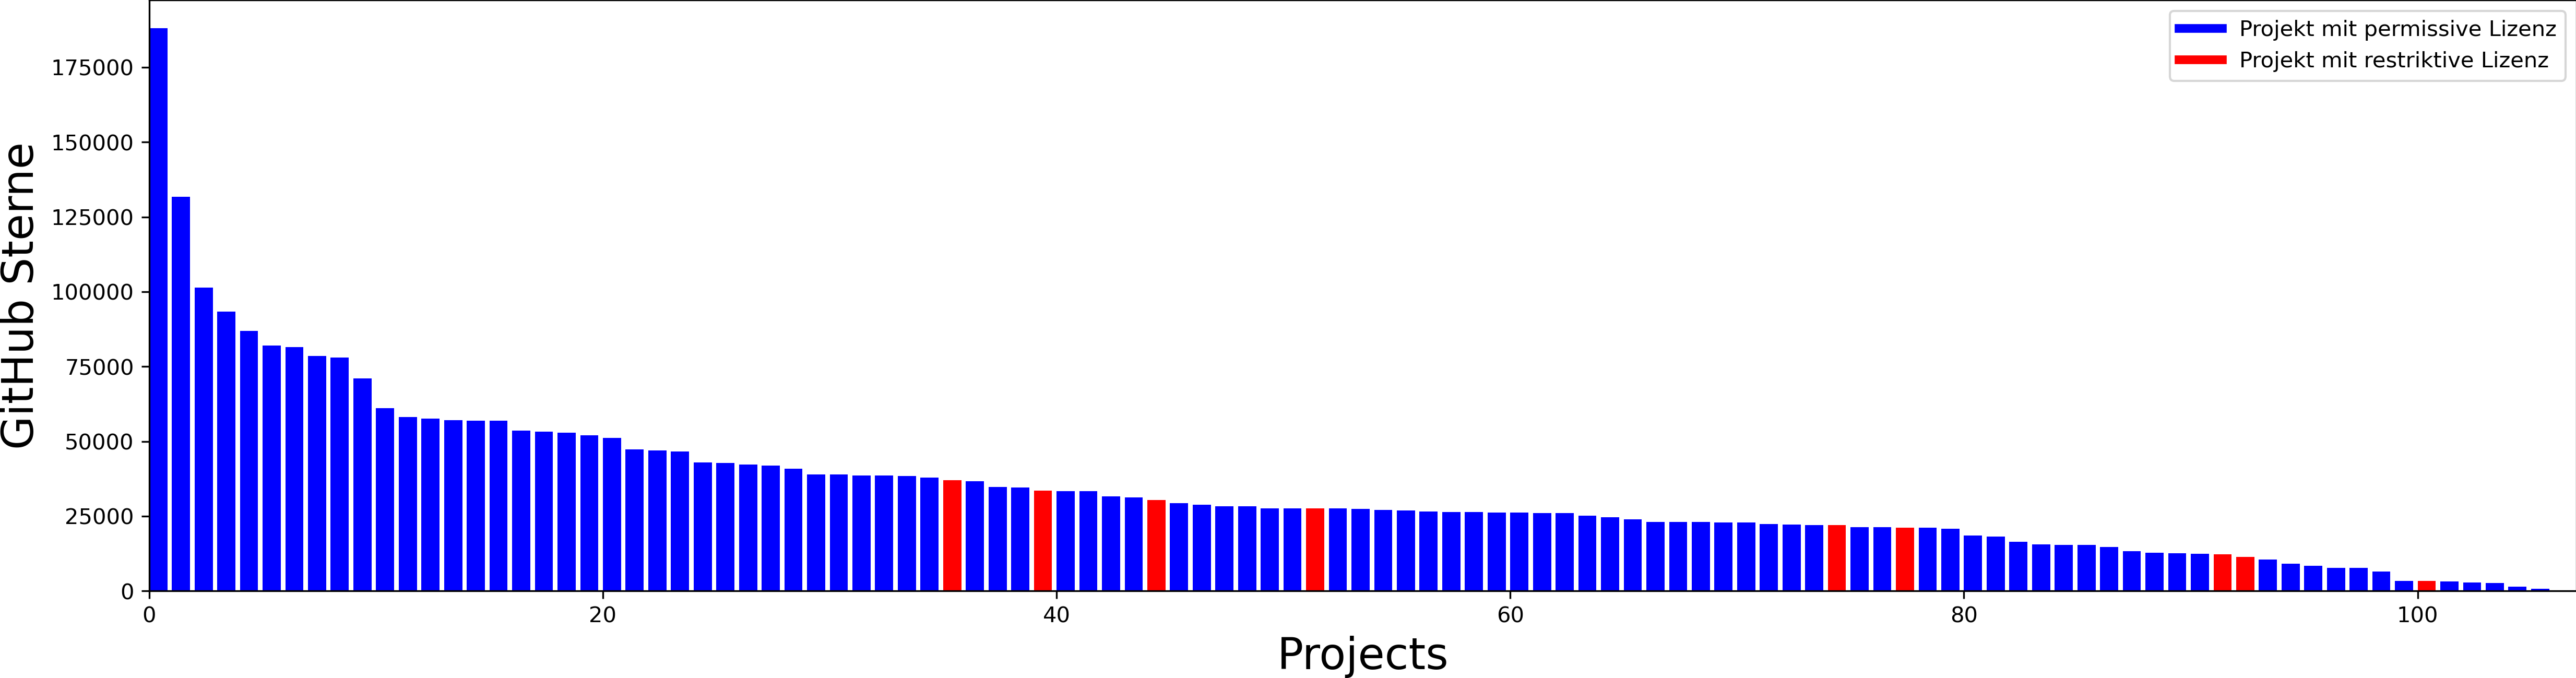
\includegraphics[scale=0.4]{figures/05/permissive_vs_restrictive_asBarChart.png}
    \caption{Effekt von Lizenzen auf GitHub Sterne}
    \label{abb:permissive_vs_restriktiv_BarChart}
\end{figure}

% Abbildung: Lizenzen vs Commits
\begin{figure}[]
    \centering
    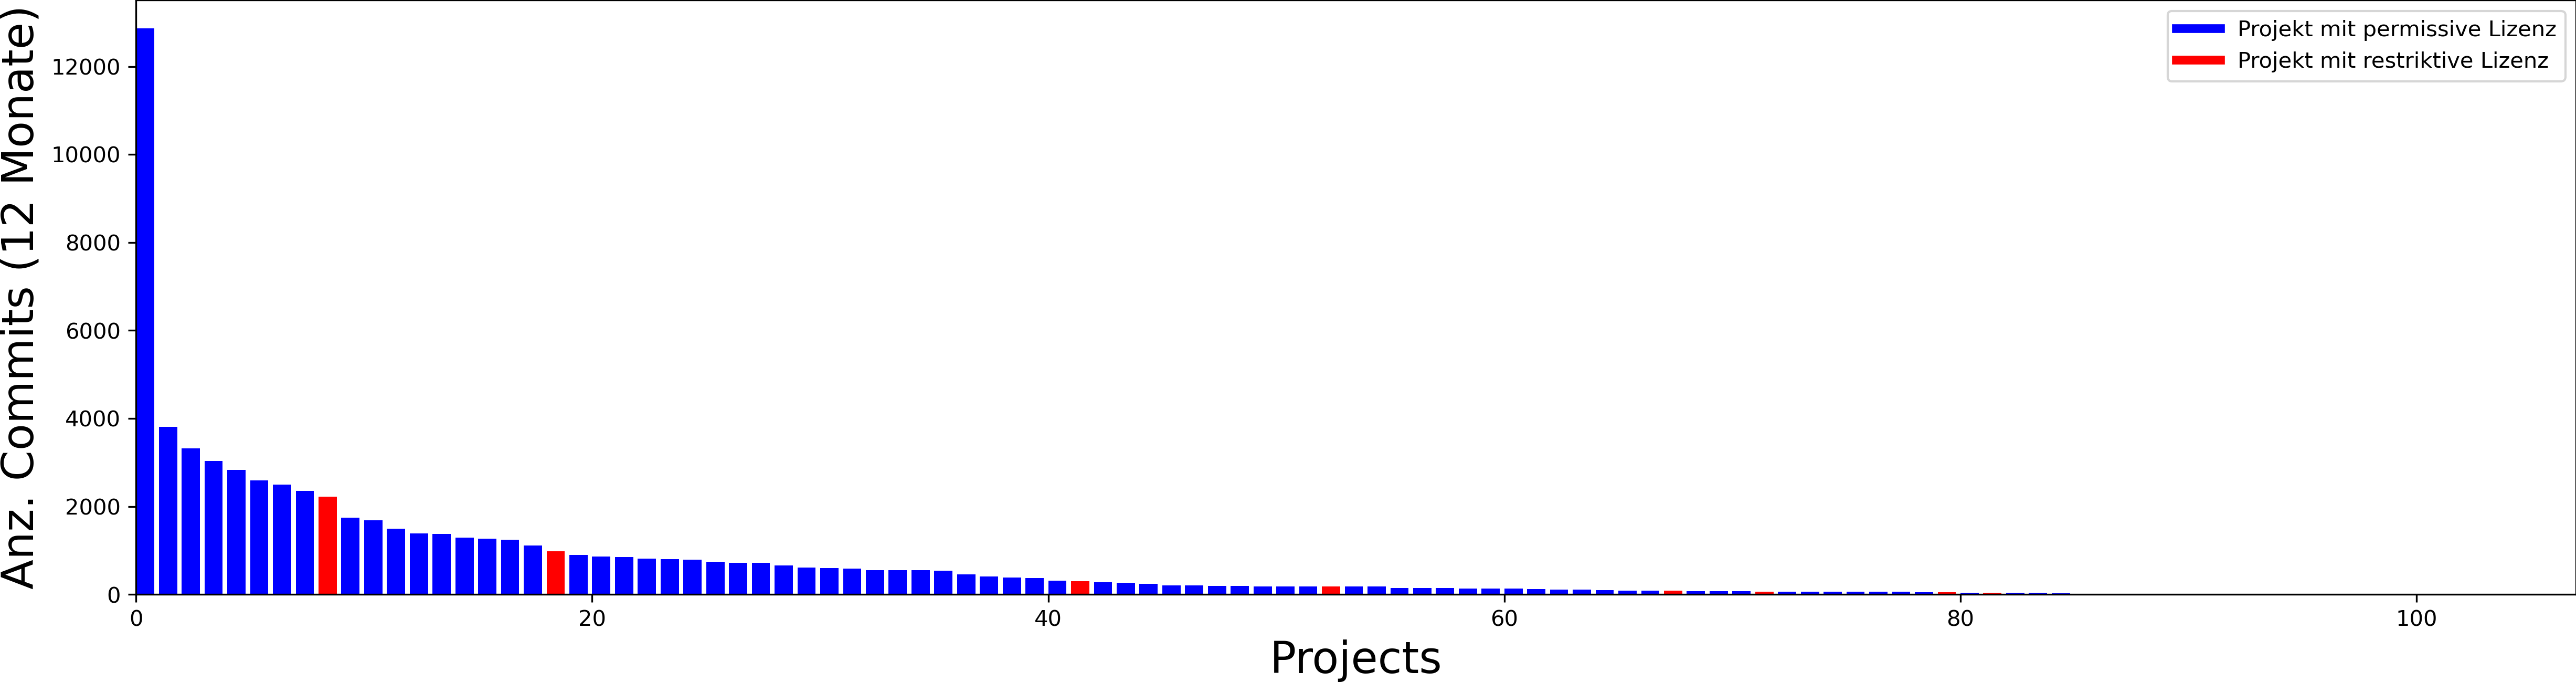
\includegraphics[scale=0.4]{figures/05/license_vs_last12MonthsCommits_asBarChart.png}
    \caption{Effekt von Lizenzen auf Anzahl der Commits}
    \label{abb:license_vs_commits}
\end{figure}



% ---------------------------------------- Code of Conduct --------------------------------------- %
\newpage %! newpage
\section{Code of Conduct}\label{sec:CoC}
Um \hyperref[H:4]{Hypothese H4} zu testen wird
der Datensatz erneut in zwei Gruppen geteilt, Projekte mit Code of Conduct und Projekte
ohne. Verglichen wurden Anzahl der Commits und Mitwirkenden mittels Median. 

Wie in Tabelle \ref{tab:relation_CoC_Popularity} zu erkennen ist, haben 53\% der Projekte einen
Code of Conduct. Im Vergleich beider Gruppen haben Projekte mit Code of Conduct 717\% mehr
Commits und 201\% mehr Mitwirkender, als Projekte ohne.


\begin{table}[h]
    \begin{tabular}{l|c|c|}
        \cline{2-3}
                                    & \multicolumn{1}{l|}{\textbf{Projekte mit Code of Conduct}} & \multicolumn{1}{l|}{\textbf{Projekte ohne Code of Conduct}} \\ \hline
        \textbf{Anzahl}             & 57                                                         & 51                                                          \\ \hline
        \textbf{Median Commits}     & 556                                                        & 68                                                          \\ \hline
        \textbf{Median Mitwirkende} & 313                                                        & 104                                                         \\ \cline{2-3}
    \end{tabular}%
    \caption{Relation von Code of Conduct und Beliebtheit}
    \label{tab:relation_CoC_Popularity}
\end{table}





% -------------------------------------- Contributing Guide -------------------------------------- %
\newpage %!newpage
\section{Contributing Guide}

Wie im Kapitel \ref{sec:CoC} wurde auch hier der Datensatz in zwei Gruppen unterteilt. Projekte mit
und ohne einen Contributing Guide (CG). Um \hyperref[H:5]{Hypothese H5} zu testen soll der Zusammenhang
zwischen dem Vorhandensein eines CG und Anzahl der Mitwirkenden bzw. Commits erforscht werden.

Anders als beim Code of Conduct, haben hier 86\% aller Projekte einen CG. Verglichen wurden erneut
der Median der Anzahl der Mitwirkenden und Anzahl der Commits, Projekte mit einem CG haben 463\% mehr
Commits und 412\% mehr Mitwirkende.

Zusätzlich werden die Projekte nach Anzahl der Mitwirkenden (sieh Abbildung \ref{abb:ContributingGuide_vs_Contributors})
sortiert, wie man erkennen kann haben die Projekte mit den meisten Mitwirkenden alle einen CG. Das
erste Projekt ohne belegt hier Platz 54. Nach dem gleichen Schema wurden auch nach Anzahl der Commits
sortiert, das erste Projekt ohne CG belegt Platz 42.
In beiden vergleichen platzieren sich Projekte mit CG weit vor Projekten ohne.

\begin{figure}[h]
    \centering
    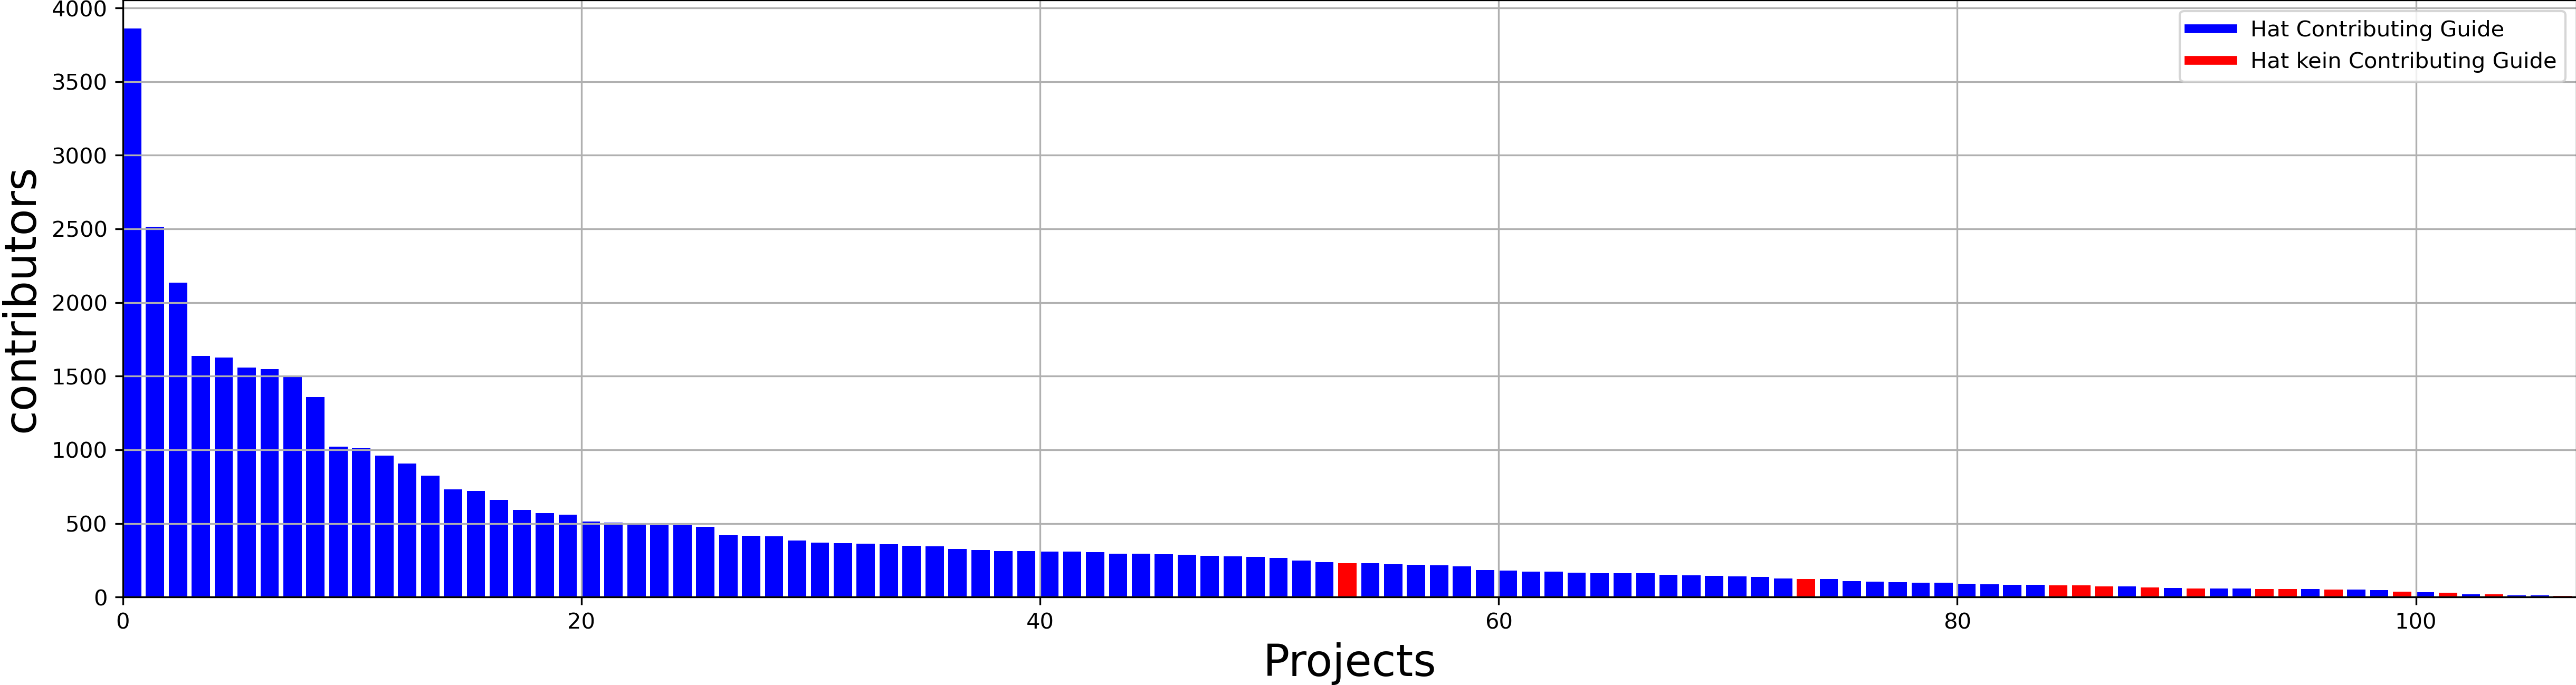
\includegraphics[scale=0.42]{figures/05/Contributors_Projects_asBarChart.png}
    \caption{Einfluss von Contributing Guide auf Mitwirkende}
    \label{abb:ContributingGuide_vs_Contributors}
\end{figure}



% ------------------------------------------- Sponsoren ------------------------------------------ %
\section{Einfluss von Sponsoren auf den technischen Erfolg}\label{sec:sponsoren_datenerhebung}


Erneut wurde der Datensatz in zwei Gruppen geteilt, Projekte mit und ohne Sponsoren. Verglichen wurde
der Median der Commits der letzten 12 Monate sowie die Anzahl an Mitwirkenden 
(Sieh Tabelle \ref{tab:Sponsors_vs_NonSponsors}).
52\% der Projekte haben Sponsoren. Projekte mit Sponsoren haben 72\% mehr Commits und 86\% mehr Mitwirkende


\begin{table}[h]
    \begin{tabular}{l|c|c|}
        \cline{2-3}
                                                      & \multicolumn{1}{l|}{\textbf{Projekte mit Sponsoren}} & \multicolumn{1}{l|}{\textbf{Projekte ohne Sponsoren}} \\ \hline
        \textbf{Anzahl der Projekte}                  & 56                                                   & 52                                                    \\ \hline
        %\textbf{Median Anz. Sterne}                   & 26.468                                               & 27.551                                                \\ \hline
        %\textbf{Median Anz. Downloads}                & 1.409.792                                            & 1.094.063                                             \\ \hline
        \textbf{Median Commits der letzten 12 Monate} & 221                                                  & 128                                                   \\ \hline
        \textbf{Median Anz. Mitwirkenden}             & 289                                                  & 155                                                   \\ \hline
    \end{tabular}%
    \caption{Relation von Sponsoren und Erfolg}
    \label{tab:Sponsors_vs_NonSponsors}
\end{table}

